\documentclass[oneside,12t]{classes/Thesis}

\usepackage[utf8]{inputenc}
\usepackage{ulem}
\usepackage[english]{babel}

\usepackage{url}
\graphicspath{{img/}}
\DeclareGraphicsExtensions{.pdf,.png}

\usepackage{fixltx2e}


\usepackage{algorithm}
\usepackage{algorithmic}
\usepackage{caption}
\usepackage{subfigure}

\title{A task based programming model for the fine-grain parallelization of sparse linear solvers}


\authorFirstName{Corentin}
\authorLastName{Rossignon}
\authorMail{corentin.rossignon@gmail.com}

\directors{Pascal \textsc{H\'{e}non}, Olivier \textsc{Aumage}, Samuel \textsc{Thibault} and Raymond \textsc{Namyst}}

\laboratory{LaBRI}
\laboratoryURL{http://www.labri.fr/}
\university{Université de Bordeaux}
\universityURL{http://www.univ-bordeaux.fr/}


\logo{bordeaux1}
\degreeDate{??th ???? 201?}
\degree{Doctor in Computer Science}
\degreeSpeciality{High Performance Computing}

\metadataSetup

% turn of those nasty overfull and underfull hboxes
\hbadness=10000
\hfuzz=50pt

\begin{document}

\dominitoc
\tikzstyle{decision} = [diamond, draw, fill=blue!20,
text width=3em, text centered, node distance=2.5cm, inner sep=0pt,font=\scriptsize]
\tikzstyle{block} = [rectangle, draw, fill=blue!20,
text width=4em, text centered, rounded corners, minimum height=1em,font=\scriptsize]
\tikzstyle{line} = [draw, thick, color=black!50,font=\scriptsize]
\tikzstyle{cloud} = [draw, ellipse,fill=red!20, node distance=2.5cm,
minimum height=0.1em,font=\scriptsize]

\maketitle

%set the number of sectioning levels that get number and appear in the contents
\setcounter{secnumdepth}{3}
\setcounter{tocdepth}{3}

\frontmatter % book mode only
\pagenumbering{roman}
%\input{src/acknowledgement}
%La résolution de grands systèmes linéaire creux est un élément essentiel des simulations numériques. Ces résolutions peuvent représenter jusqu'à 80\% du temps de calcul des simulations.
Une parallélisation efficace des noyaux d'algèbre linéaire creuse conduira donc à obtenir de meilleurs performances. En mémoire distribuée, la parallélisation de ces noyaux se fait le plus souvent en modifiant le schéma numérique. Par contre, en mémoire partagée, un parallélisme plus efficace peut être utilisé. Il est donc important d'utiliser deux niveaux de parallélisme, un premier niveau entre les noeuds d'une grappe de serveur et une deuxième niveau à l'intérieur du noeud. Lors de l'utilisation de méthodes itératives en mémoire partagée, les graphes de tâches permettent de décrire naturellement le parallélisme en prenant comme granularité le travail sur une ligne de la matrice. Malheureusement, cette granularité est trop fine et ne permet pas d'obtenir de bonnes performances.
Dans cette thèse, nous allons étudier le problème de la granularité pour la parallélisation par graphe de tâches. Nous proposerons d'augmenter la granularité des tâches de calcul en créant des agrégats de tâches qui deviendront eux-mêmes des tâches. L'ensemble de ces agrégats et des nouvelles dépendances entre les agrégats formera un graphe de granularité plus grossière. Ce graphe sera ensuite utilisé par un ordonnanceur de tâches pour obtenir de meilleurs résultats. Nous utiliserons comme exemple la factorisation ILU d'une matrice et nous montrerons les améliorations apportées par cette méthode. Dans un second temps, nous nous concentrerons sur les machines à architecture NUMA. Dans le cas de l'utilisation d'algorithmes limités par la bande passante mémoire, il est intéressant de réduire les effets NUMA liés à cette architecture. Nous montrerons comment prendre en compte ces effets dans un intergiciel à base de tâches pour améliorer les performances d'un programme.

Mots-clés : parallélisme, graphe de tâches, supports d’exécution, NUMA, multi-coeurs, algèbre linéaire creuse

%Solving large sparse linear system is an essential part of numerical simulations. These resolve can take up to 80\% of the total of the simulation time.
An efficient parallélization of sparse linear kernels inéaire creuse leads to obtain better performances. In distributed memory, parallélization of theses kernels are often done by changing the numerical scheme. Par contreContrariwise, in shared memory, a more efficient parallelism can be used. It's significant to use two levels of parallelism, a first one between nodes of a cluster and a second inside a node. Lors de l'utilisation de méthodes itératives en mémoire partagée, les graphes de tâches permettent de décrire naturellement le parallélisme en prenant comme granularité le travail sur une ligne de la matrice. Malheureusement, cette granularité est trop fine et ne permet pas d'obtenir de bonnes performances.
Dans cette thèse, nous allons étudier le problème de la granularité pour la parallélisation par graphe de tâches. Nous proposerons d'augmenter la granularité des tâches de calcul en créant des agrégats de tâches qui deviendront eux-mêmes des tâches. L'ensemble de ces agrégats et des nouvelles dépendances entre les agrégats formera un graphe de granularité plus grossière. Ce graphe sera ensuite utilisé par un ordonnanceur de tâches pour obtenir de meilleurs résultats. Nous utiliserons comme exemple la factorisation ILU d'une matrice et nous montrerons les améliorations apportées par cette méthode. Dans un second temps, nous nous concentrerons sur les machines à architecture NUMA. Dans le cas de l'utilisation d'algorithmes limités par la bande passante mémoire, il est intéressant de réduire les effets NUMA liés à cette architecture. Nous montrerons comment prendre en compte ces effets dans un intergiciel à base de tâches pour améliorer les performances d'un programme.

Mots-clés : parallélisme, graphe de tâches, supports d’exécution, NUMA, multi-coeurs, algèbre linéaire creuse

\tableofcontents
\mtcaddchapter
\mainmatter % book mode only



%=========================================================
\chapter{Context : Simulate petroleum extraction}
\minitoc
\vspace{1cm}
%=========================================================

%+++++++++++++++++++++++++++++++
\section{Reservoir simulation}
%-------------------------------
\subsection{Overview}
  \begin{itemize}
    \item Explain what is a reservoir
    \item What is it use for ?
  \end{itemize}
%-------------------------------
\subsection{From physics to computation}
  \begin{itemize}
    \item Rapid transition between physical model to sparse non-linear system
    \item Explain newton
  \end{itemize}
%+++++++++++++++++++++++++++++++


%+++++++++++++++++++++++++++++++
\section{Linear algebra}
%-------------------------------
\subsection{Dense linear algebra}
  \begin{itemize}
    \item Well studied in HPC
    \item Performance don't scale with problem size
  \end{itemize}
%-------------------------------
\subsection{Sparse linear algebra}
  \begin{itemize}
    \item Explain format and computation problem (bandwidth, ...)
    \item Allow to solve large problem
  \end{itemize}
%+++++++++++++++++++++++++++++++


%+++++++++++++++++++++++++++++++
\section{Solving large sparse linear system}
%-------------------------------
\subsection{GMRES}
  \begin{itemize}
    \item Iterative method for general matrix
    \item Doesn't work well with our matrices
  \end{itemize}
%-------------------------------
\subsection{Preconditioned GMRES}
  \begin{itemize}
    \item Need to add a ILU part which is not parallel
    \item Improve a lot convergence of our matrices
  \end{itemize}
%-------------------------------
\subsection{Domain decomposition}
  \begin{itemize}
    \item Can be use to obtain complete parallel part
    \item Degrade convergence
  \end{itemize}
%-------------------------------
\subsection{Reservoir case studies}
  \begin{itemize}
    \item SPE10, often use in reservoir benchmark
    \item generate
    \item ordering -> change preconditionner performance
  \end{itemize}
%+++++++++++++++++++++++++++++++



%+++++++++++++++++++++++++++++++
\section{Computers to target}
%-------------------------------
\subsection{SMP}
  \begin{itemize}
    \item Memory don't scale with a high number of core
  \end{itemize}
%-------------------------------
\subsection{NUMA}
  \begin{itemize}
    \item Memory scale with a high number of core
    \item Need to add some support in program to obtain performance
  \end{itemize}
%-------------------------------
\subsection{Many-core}
  \begin{itemize}
    \item Xeon phi
    \item GPU ?
    \item Too many change in program but not always performance (data transfer)
  \end{itemize}
%-------------------------------
\subsection{Our computers}
\subsubsection{Rostand}
  \begin{itemize}
    \item Bi-socket
    \item NUMA
    \item 12 Cores
    \item MPI
  \end{itemize}
\subsubsection{Manumanu}
  \begin{itemize}
    \item 20 sockets
    \item NUMA
    \item Altix UV100
    \item 160 Cores
  \end{itemize}
%+++++++++++++++++++++++++++++++

%+++++++++++++++++++++++++++++++
\section{Multi-core parallelism}
%-------------------------------
\subsection{Parallel for loop}
  \begin{itemize}
    \item OpenMP
  \end{itemize}
%-------------------------------
\subsection{Task paradigm}
  \begin{itemize}
    \item PaRSEC
    \item
  \end{itemize}
%+++++++++++++++++++++++++++++++


\subsection{Runtime}
A runtime is a piece of software used by others software to abstract part of the system.
%
There are several type of runtime.
%
Some high level programming languages use runtime, for example Java has a runtime for garbage collection.
%
Also some implementations of MPI have a runtime.
%
Task based programming also tend to have a runtime.
%
In the following part, we will focus on runtime support for task based programming.



The main interest of runtime in task based programming is to schedule tasks while respecting strict dependencies order.
%Le rôle des supports d'exécution pour la programmation en tâches est d'orchestrer la réalisation des tâches en respectant leurs dépendances.
%
These runtimes also provide a load balancing over all available hardware ressources (potentially heterogeneous) while keeping data consistency.
%Ils se chargent de la répartition des tâches sur les ressources matérielles disponibles (potentiellement hétérogènes) tout en assurant la cohérence des données.
%
Some runtime also provide memory transfer between ressources, for example between main memory and a graphical card or just between two processes.
%
These transfers could be implicit, the runtime has data knowledge, or they could be explicit, a special task.


Some runtime use schedule policy (static or dynamic) to improve load balancing.
%
But the perfect scheduler doesn't exist maybe will never exist.
%
Indeed, finding the best schedule for a set of tasks on a limited number of resources machine is a NP-complete problem\footnote{A problem is NP-complete if the solving time is polynomial compare to input data.}.
%
Some heuristic are used to obtain some reasonably good results, for example the greedy algorithm.
%
Also, some heuristic needs more information about tasks, like an estimated cost.


\subsection{Timeline of runtime}
Back in 80's, some scientist succeed in interconnecting some processors together and obtain a parallel machine,

A new idea appears to make scheduler , it's name is {\em work-stealing}.
La notion de vol de tâches (en anglais \textit{work-stealing}) apparaît ensuite, ce qui rend les ordonnanceurs dynamiques.
%
With this idea, tasks can be schedule during run-time, when a hardware resource is free.
%
One of the best example is Cilk~\cite{Cilk}, first published in 1994 and still developed under the Cilk++~\cite{Cilk++}.
%
Tasks are describe by the programmer with additional keywords to the C language, for example in Cilk the keyword {\em spawn} before a function call means that a task must be create and the runtime can schedule it.
%
In the case of Cilk a specific compiler must be use in order to transform the code into a set runtime call, this is close of source-to-source compiler.
%
The parallelism that consist in spawning tasks and then wait for some of them is often called {\em insert task} paradigm.
%
One can also used the name {\em sequential task graph} because the task graph is build along the computation.
%
On the opposite, one can found {\em Parametrized Task Graph} or in a shorter way {\em PTG} where the graph .

OpenMP~\cite{OpenMP} is a different from above, it is a runtime specialized in loop parallelism without data dependency.
%
Somewhat like Cilk, it uses some language extension ({\em \#pragma omp <action>} in C) and a specific compiler must be used to translate the code (transform the loop into a function and call the right runtime functions).
%
In 1997, the specification 3.0 of OpenMP add the keyword {\em task} to support {\em sequential task graph}, it still doesn't support implicit data dependencies.
%
More recently, the specification 4.0 add an support of implicit data dependencies.
%
To date, OpenMP is certainly the most commonly used runtime through that one can obtain a parallel application with the simple well know line {\em \#pragma omp parallel for}


At begin of 2000's, architecture in the processor became parallel.
%
Two or more cores cohabit on a single chip and share some resources like cache or memory bandwidth.
%
One can have multi threading parallelism, but there is need of runtime to exploit this parallelism.
%
For example, Intel TBB (\textit{Threading Building Blocks})~\cite{TBB} which is developed by Intel since 2006 especially for abstract multi-core programming and with the same goal SMPSs~\cite{SMPSs}(now part of STARSs, see below) since 2007.

When we use a cluster, there is two choice.
%
On the one hand, there is DSM\footnote{Distributed Shared Memory}, which is very simple to use but
%
On the other hand, there is message passing paradigm, which is more difficult to use but give good result.
%
It is the most used paradigm for distributed memory especially with the MPI norm.
%

More recently, in the late 2000's, the GPGPU revolution leads the apparition of new type of runtime.
%
These runtimes must now support heterogeneous resources with sometimes several address spaces.
%
They must also integrate a support to automatically transfer data between the several address space.
%
Among these runtimes, one can found StarPU~\cite{ATNW2011,Aug2011}, PaRSEC~\cite{PaRSEC} (formerly called DAGuE~\cite{DAGuE2012}), X-KAAPI~\cite{X-KAAPI} and STARSs (became OMPSs~\cite{OMPSs} by the merge of SMPSs, ClusterSs and CellSs,\dots).

Some runtime specialized in loop parallelism also gain a GPU support, like OpenMP in is specification 4.0.
%
But this specification is mostly inspired from OpenACC~\cite{OpenACC} which wants to simplify parallel programming of heterogeneous CPU/GPU systems.

Meanwhile, Intel prepare a against GPU, the {\em Kinghts Corner}.
%
A PCI express card with around 60 cores with the well known architecture x86, more precisly an old pentium architecture with a very powerful SIMD unit.
%
The main advantage of this architecture, is that the card can be seen as a computer with 60 cores totally independent because a standard kernel can run inside.
%
So almost all runtime are directly compatible or just need minor changes.



\subsection{Classification of runtime}
We can try to classify all these runtime by functionality, we can consider three form of parallelism expression : loop parallelism, PTG and insert task paradigm.
%
The first table~\ref{tab:runtime_family} summarizes capabilities of a set of runtime, a {\it ++} entry means that the capacity is often put forward in publication, a single {\it +} means that the runtime has the functionality but it is not a major advantage of the runtime.
%
The second table~\ref{tab:runtime_archi} summarizes target architecture of the same set of runtime.
%
In the case of distributed memory, we can see two method to address this problem.
An implicit method when the runtime has a memory manager and can do automatic transfer.
Or an explicit method often describe as user task, some runtime, like StarPU, support asynchronous transfer, without this support the explicit method is less efficient.


We can also try to differentiate other differences, like the use of an API ({\it Application Programming Interface}) or the use of a source-to-source compiler.
%
Data management is also important in a runtime to optimize data transfer between CPU and GPU, or between two CPUs.

\begin{table}[h!]
\centering
\begin{tabular}{c|ccc}
  \textit{runtime}& loop parallelism & PTG & Insert task\\
  \hline
        Cilk           &    &    & ++ \\
        Cilk++         & ++ &    & ++ \\
        OpenMP $<$ 3.0 & ++ &    &    \\
        OpenMP 3.x     & ++ &    & +  \\
        OpenMP 4.0     & ++ &    & +  \\
        OpenACC        & ++ &    & +  \\
        Intel TBB      & +  &    & ++ \\
        OMPSs          & +  &    & ++ \\
        Intel CnC      & +  & ++ &    \\
        PaRSEC         &    & ++ &    \\
 PGAS(coarray fortran) & ++ &    &    \\
        StarPU         &    &    & ++ \\
        KAAPI          & ++ &    &    \\
        X-KAAPI        & +  &    & ++
\end{tabular}
\caption{Classification of runtime by capabilities}
\label{tab:runtime_family}
\end{table}

\begin{table}[h!]
\centering
\begin{tabular}{c|ccc}
  \textit{runtime} & Shared memory & Distributed memory & GPU accelerator \\
\hline
        Cilk           & X &           &   \\
        Cilk++         & X &           &   \\
        OpenMP $<$ 3.0 & X &           &   \\
        OpenMP 3.x     & X &           &   \\
        OpenMP 4.0     & X &           & X \\
        OpenACC        & X &           & X \\
        Intel TBB      & X &           &   \\
        OMPSs          & X & explicit  & X \\
        Intel CnC      & X & implicit  &   \\
        PaRSEC         & X & implicit  &   \\
 PGAS(coarray fortran) & X & implicit  &   \\
        StarPU         & X & implicit/explicit  & X \\
        KAAPI          & X &           & X \\
        X-KAAPI        & X & explicit  & X
\end{tabular}
\caption{Classification of runtime by supported architecture}
\label{tab:runtime_archi}
\end{table}





%=========================================================
\chapter{A problem of granularity}
\minitoc
\vspace{1cm}
%=========================================================
%+++++++++++++++++++++++++++++++
\section{Parallelize preconditioned GMRES}
%-------------------------------
\subsection{GMRES algorithm}
  \begin{itemize}
    \item Explain GMRES algorithm
    \item it is mostly parallel for BLAS1 and BLAS2
    \item We need to use a preconditionner
  \end{itemize}
%-------------------------------
\subsection{Incomplete LU}
  \begin{itemize}
    \item Explain ILU
    \item It can be parallel...
    \item ... but a lot of data dependencies
    \item and small tasks, a granularity problem
  \end{itemize}
%-------------------------------
%+++++++++++++++++++++++++++++++

%+++++++++++++++++++++++++++++++
\section{Why granularity is so important ?}
%-------------------------------
\subsection{Parallelism vs overhead}
  \begin{itemize}
    \item Talk about runtime overhead
    \item Give some result without aggregation
  \end{itemize}
%-------------------------------
\subsection{Current solutions}
  \begin{itemize}
    \item X-KAAPI
    \item SCOOP
    \item Capsules
    \item for each explain why they don't fit our problem
  \end{itemize}
%+++++++++++++++++++++++++++++++


%+++++++++++++++++++++++++++++++
\section{My solution to our granularity problem}
%-------------------------------
\subsection{Taggre : a task aggregator framework}
%-------------------------------
\subsection{Aggregate operators}
  \begin{itemize}
    \item Put tasks together without making cycle in DAG
  \end{itemize}
%-------------------------------
\subsubsection{Sequential}
\subsubsection{Front}
\subsubsection{Depth front}
\subsubsection{Continuation oriented}
%-------------------------------
\subsection{Examples of strategies}
  \begin{itemize}
    \item Talk about the 7 dwarfs (\url{http://view.eecs.berkeley.edu/wiki/Dwarf_Mine})
  \end{itemize}
%+++++++++++++++++++++++++++++++




%+++++++++++++++++++++++++++++++
\section{Results}
%-------------------------------
\subsection{Factorization and Triangular solve improvement}
  \begin{itemize}
    \item Explain why we benchmark this part
    \item Try a lot of coarse string
  \end{itemize}
%-------------------------------
\subsection{Aggregation overhead}
  \begin{itemize}
    \item Explain why it isn't a real problem
    \item Give some numbers
  \end{itemize}
%-------------------------------
\subsection{Subdomain decomposition}
  \begin{itemize}
    \item Explain why it isn't a real problem
    \item Give some numbers
    \item Talk about bandwidth
  \end{itemize}
%-------------------------------
\subsection{Discussion}
  \begin{itemize}
    \item Compare domain with domain decomposition
  \end{itemize}
%+++++++++++++++++++++++++++++++





%=========================================================
\chapter{Memory bandwidth limitation}
\minitoc
\vspace{1cm}
%=========================================================
\subsection{Deux fois plus de coeurs mais pas deux fois plus rapide}
Comme dit dans le chapitre précédent, l'algorithme du GMRES se parallélise bien parce qu'il est essentiellement composé d'opérations sur des vecteurs.
%
L'opération la plus coûteuse est le produit d'une matrice par un vecteur (SpMV).
%
Notre implémentation du SpMV est optimisée pour prendre en compte la structure bloc des entrées de la matrice quand le nombre de variables primaires est supérieur à 1.
%
Dans ce cas, nous pouvons réutiliser des données en cache.
%
Malgré ces optimisations, le SpMV est toujours limité par la bande passante mémoire.
%
Les courbes d'accélération du SpMV nous montrent que le gain de performance n'est pas linéaire avec le nombre de coeurs (Fig.~\ref{fig:res_spmv_omp_rostand})..
%
Le constat est même pire que ça, on arrive difficilement à une accélération de 2 sur 12 coeurs lorsqu'on utilise une seule variable primaire.
%
Si l'on regarde les compteurs matériels, on s'aperçoit que la moitié de la bande passante de chaque banc NUMA est utilisée par des accès distant.
%
Donc environ la moitié des accès mémoires sont faits une plus grande latence.

%   (-_-)   %
\begin{figure}[t!]
  \centering
  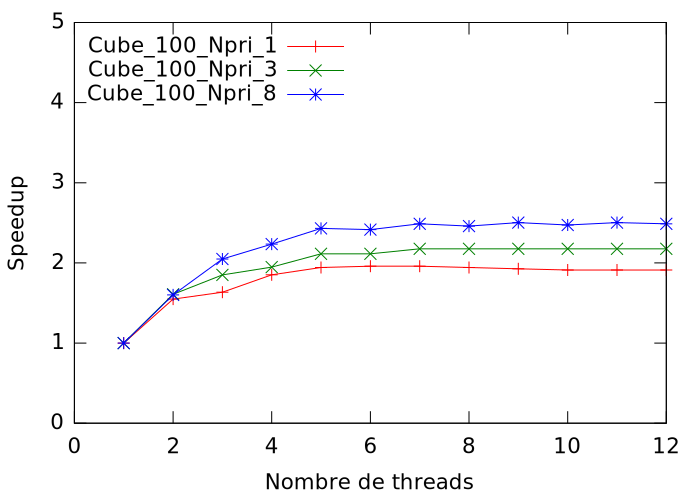
\includegraphics[width=0.7\textwidth]{res_spmv_omp}
  \caption{Accélération du produit matrice vecteur creux sur Rostand en mémoire partagée.}
  \label{fig:res_spmv_omp_rostand}
\end{figure}

%+++++++++++++++++++++++++++++++
\section{Current NUMA management}
In a general way, a program allocates memory from a virtual address space split into pages.
%
Each pages used by the program is transparently mapped by the Operating System to a physical memory location.
%
Thus, some virtual pages can also be moved from one physical location to another one, while the virtual/physical mapping is transparently updated accordingly to the Operating System without affecting the execution of user level programs.
%
However, the physical location of virtual page may impact the program performance on NUMA architectures, depending on the connectivity between the physical memory bank where a page is located and the socket core that is accessing this memory bank.
%
The NUMA memory allocation policy is defined by the kernel of the Operating System.
%
With Linux, at least the following three memory policies are generally available:
\begin{itemize}
        \item {\em First Touch}: Memory is allocated on the bank next to the core which accessed the data first.
                         This is the default policy.
        \item {\em Bind}: Memory is allocated on a specific bank.
        \item {\em Interleaved}: Memory allocations are interleaved among all the banks available.
\end{itemize}
On Linux, these policies can be set either through the \textit{mbind} system call, or with the {\em numactl} command line tool.
%
A new mechanism also come with the version 3.13 of Linux, AutoNUMA.
%
This mechanism use page fault trapping which has a non negligible overhead.
%
AutoNUMA can only be configured at system level with root privilege and for all applications.


Other operating system may come with their own specific sets of NUMA memory allocation policies.
%
Solaris, for instance, also provides the \textit{next-touch}~\cite{next_touch} policy.
%
When this policy is selected, a memory page is moved to the bank close to the core that subsequently accesses it.


%-------------------------------
\subsection{First touch}
This is the default policy on Linux.
%
When a thread wants to access to a not yet mapped virtual memory page, the kernel allocate a new physical page near to the thread.
%
The idea behind this policy isn't bad, a memory page is often use by one thread.
%
So when a thread touch a page for the first time, it may continue to work with this page and this page must be close to the thread.
%
But some threaded program doesn't work in that way.
%
Let's imagine the case that in a program the setup phase which allocate all pages isn't multithreaded.
%
In that case, all pages are allocated on the same NUMA node, close to the thread which have done the setup.


%-------------------------------
\subsection{Interleaved memory}
When the interleaved policy is selected, the kernel uniformly distributes newly allocated physical pages among all available NUMA banks, following a round robin scheme.
%
While having very little impact on the applicative code, the interleave policy often shows some effectiveness in mitigating NUMA overheads in the general case.
%
In average, the latency doesn't change too much but thease because of pages Because it distributes the required memory bandwidth over the various memory banks.
%
Thus, it is usually worthwhile to experiment with it, before investigating the NUMA issue further.


While the results we obtain show an improved speed-up with TBB and interleaved policy,
it should be noted that sequential runs with interleaved policy are of
course worse, because of memory access penalties introduced by NUMA.
%% Parallel runs however show a better speed-up.
When comparing
interleaved page allocation with first-touch allocation, we get
an average improvement of 3.5\,\% on ILU(k) preconditioner
and 6.2\,\% on triangular solve with two 4-core sockets.

These improvements could be further enhanced by taking into account the locality of data
used by tasks within the task scheduler. This is the purpose of the
following section.



%-------------------------------
\subsection{Next-touch}
%-------------------------------
\subsection{Automatic solution}
%-------------------------------
\subsection{One MPI per NUMA bank}
%+++++++++++++++++++++++++++++++


%+++++++++++++++++++++++++++++++
\section{Handle NUMA directly in scheduler}
%-------------------------------
\subsection{Status of current scheduler}
  \begin{itemize}
    \item PaRSEC : one vp per NUMA
  \end{itemize}
%-------------------------------
\subsection{NATaS : schedule tasks on NUMA}
  \begin{itemize}
    \item bind task to a processor
    \item allow NUMA work-stealing
    \item bind memory pages
  \end{itemize}
%+++++++++++++++++++++++++++++++


%+++++++++++++++++++++++++++++++
\section{Results}
%-------------------------------
\subsection{Factorization and Triangular solve}
  \begin{itemize}
    \item Support NUMA in tasks
  \end{itemize}
%-------------------------------
\subsection{Sparse matrix vector multiplication}
  \begin{itemize}
    \item problem of SpMV
  \end{itemize}
%-------------------------------
\subsection{First touch}
results
%-------------------------------
\subsection{Interleave}
results
%-------------------------------
\subsection{Automatic NUMA balancing}
  \begin{itemize}
    \item Results on personal machine
    \item very recent kernel
  \end{itemize}
%-------------------------------
\subsection{NATaS}
results
%-------------------------------
\subsection{Discussion}
  \begin{itemize}
    \item Interleave isn't so bad on bi-socket,...
    \item NATaS always give best result
    \item Maybe NATaS isn't the good answer (better scheduler or MPI)
  \end{itemize}
%+++++++++++++++++++++++++++++++


%=========================================================
\chapter{The fork and join syndrome}
\minitoc
\vspace{1cm}
%=========================================================
%+++++++++++++++++++++++++++++++
%\section{Data dependencies}
%-------------------------------
%\subsection{Implicit dependencies}
%-------------------------------
%\subsection{Explicit dependencies}
%+++++++++++++++++++++++++++++++


%+++++++++++++++++++++++++++++++
\section{The fork and join syndrome}
%-------------------------------
\subsection{How to see it ?}
  \begin{itemize}
    \item Show that we have too much synchronization (Paje trace)
  \end{itemize}
%-------------------------------
\subsection{Domain decomposition and overlap}
  \begin{itemize}
    \item Explain what domain decomposition and overlap is
  \end{itemize}
%+++++++++++++++++++++++++++++++


%+++++++++++++++++++++++++++++++
\section{Pipeline GMRES steps}
  \begin{itemize}
    \item explain the solution to merge graph of task
  \end{itemize}
%+++++++++++++++++++++++++++++++


%+++++++++++++++++++++++++++++++
\section{Results}
%-------------------------------
\subsection{Without MPI}
  \begin{itemize}
    \item Almost no gain because no many sync
  \end{itemize}
%-------------------------------
\subsection{With MPI}
  \begin{itemize}
    \item Gain when increase number of MPI process
  \end{itemize}
%-------------------------------
\subsection{Discussion}
%+++++++++++++++++++++++++++++++




%=========================================================
\chapter{Conclusions and perspectives}
\minitoc
\vspace{1cm}
%=========================================================
%+++++++++++++++++++++++++++++++
\section{Conclusion}
  \begin{itemize}
    \item Coarsening allow us to parallelize problems with very small computation per task
    \item Improve bandwidth thanks to NUMA architecture
  \end{itemize}
%+++++++++++++++++++++++++++++++


%+++++++++++++++++++++++++++++++
\section{Perspectives}
  \begin{itemize}
    \item Automatic coarse tuning
  \end{itemize}
%+++++++++++++++++++++++++++++++



\backmatter % book mode only
%\bibliographystyle{alpha}
%\bibliography{anrt}
\appendix

\bibliographystyle{plainnat}
\bibliography{thesis}
\end{document}
